\documentclass[tikz]{standalone}
\usetikzlibrary{calc}

\begin{document}
  
\definecolor{mygreencolor}{RGB}{133,196,96}  

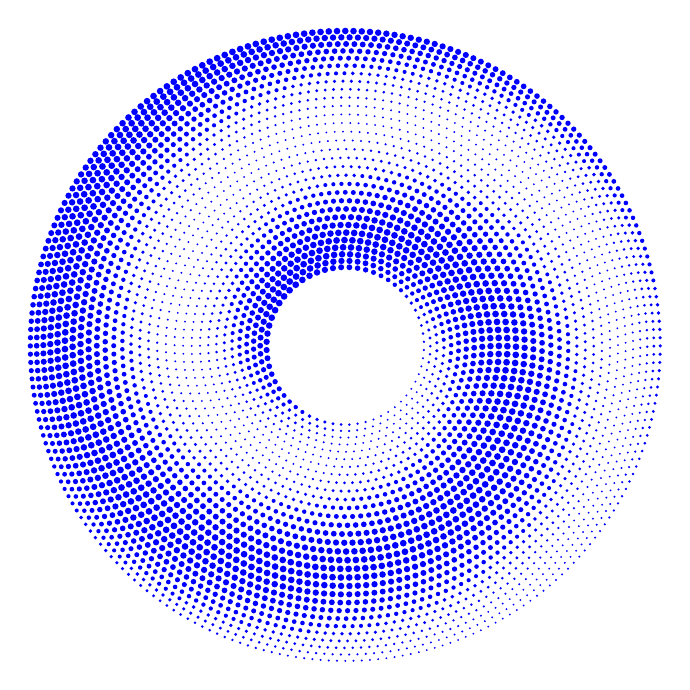
\begin{tikzpicture}

\pgfmathsetmacro\maxradius{.3}
\pgfmathsetmacro\inner{10}
\pgfmathsetmacro\outer{40}
\pgfmathsetmacro\range{\outer-\inner}

\foreach \stepy in {\inner, ..., \outer}
    \pgfmathsetmacro\stepstart{60/\stepy}
    \pgfmathsetmacro\steplast{360-\stepstart}
    \pgfmathsetmacro\stepcount{floor(360/\stepstart)} 
    \foreach \stepx in {0, \stepstart, ..., \steplast}
        \pgfmathsetmacro\stepsingle{floor(\stepx/\stepstart)}
        \pgfmathsetmacro\stepradius{(\maxradius/2)*sin(deg(\stepsingle*pi/(\stepcount/2) - pi - (\stepy/5))) + (\maxradius/2)+0.13}
        \pgfmathsetmacro\mybase{90*(\stepy-\inner)/\range)}
        \pgfmathsetmacro\mycoef{((1-cos(\mybase)+sin(\mybase))/2}
        \pgfmathsetmacro\mystepy{\inner+\range*\mycoef}
        \fill[blue] ({-(\stepx+.25*\stepcount)}:-\mystepy mm) circle (\stepradius mm);

\end{tikzpicture}

\end{document}

